\documentclass[12pt,a4paper]{article}

% Packages
\usepackage{geometry}
\geometry{margin=1in}
\usepackage{fancyhdr}
\usepackage{titlesec}
\usepackage{listings}
\usepackage{xcolor}
\usepackage{graphicx}

% Header & Footer
\pagestyle{fancy}
\fancyhf{}
\rhead{DBT - Assignment 3}
\lhead{Kamithkar Vinod}
\cfoot{\thepage}

% Title formatting
\titleformat{\section}{\large\bfseries}{Problem \thesection:}{0.5em}{}
\titleformat{\subsection}[runin]{\bfseries}{Code:}{0.5em}{}[---]
\titleformat{\subsubsection}[runin]{\bfseries}{Output:}{0.5em}{}[---]

% SQL language definition for listings
\lstdefinelanguage{SQL}{
  morekeywords={
    SELECT, FROM, WHERE, GROUP, BY, ORDER, ASC, DESC, JOIN, ON, AS,
    AND, OR, NOT, IN, IS, NULL, LIKE, HAVING, COUNT, SUM, AVG, MIN, MAX,
    CREATE, TABLE, INSERT, INTO, VALUES, UPDATE, SET, DELETE, DISTINCT,
    CASE, WHEN, THEN, ELSE, END, BETWEEN, EXISTS, UNION, ALL, ANY, LEFT,
    RIGHT, INNER, OUTER, LIMIT, OFFSET, PROCEDURE, BEGIN
  },
  sensitive=false,
  morecomment=[l]{--},
  morestring=[b]',
}

\lstset{
    language=SQL,
    basicstyle=\ttfamily\small,
    keywordstyle=\color{blue}\bfseries,
    commentstyle=\color{gray}\itshape,
    stringstyle=\color{red},
    showstringspaces=false,
    frame=single,
    breaklines=true,
    numbers=none
}

% Document Start
\begin{document}

% Title Page
\begin{center}
    \LARGE \textbf{Assignment - 3} \\[0.5cm]
    \Large \textbf{DBMS} \\[1cm]

    \begin{tabular}{rl}
        \textbf{Name:} & Kamithkar Vinod \\
        \textbf{Course:} & PG DAC AUGUST 2025 \\
        \textbf{PRN:} & 250850320040 \\
        \textbf{Form No:} & 250500480 \\
        \textbf{Date:} & 23-10-2025 \\
    \end{tabular}
\end{center}

\vspace{1cm}
\hrule
\vspace{0.5cm}

% Problems

% 1
\section{}
\textbf{Task:} Create a procedure to reset all employee salaries to 50000.

\subsection{}
\begin{lstlisting}
delimiter //
create procedure ResetAllSalaries()
begin
    update employees
    set salary = 50000
    where empid > 0;
end //
delimiter ;

call ResetAllSalaries();

select * from employees;
\end{lstlisting}

\subsubsection{}
\begin{center}
    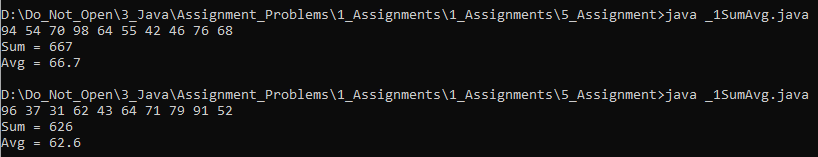
\includegraphics[width=0.8\textwidth]{1.png}
\end{center}

% 2

\section{}
\textbf{Task:} Create a procedure to delete all employees in the HR department.

\subsection{}
\begin{lstlisting}
delimiter //
create procedure delete_hr_emp()
begin
    delete from employees
    where department = 'hr';
end //
delimiter ;

call delete_hr_emp();

select * from employees;
\end{lstlisting}

\subsubsection{}
\begin{center}
    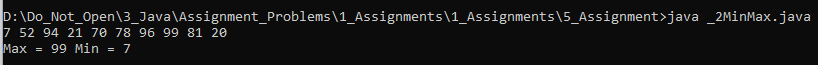
\includegraphics[width=0.8\textwidth]{2.png}
\end{center}

% 3

\section{}
\textbf{Task:} Create a procedure to increase all employee salaries by 5%.

\subsection{}
\begin{lstlisting}
delimiter //
create procedure inc_sal()
begin
    update employees 
    set salary = salary + salary * (5/100);
end //
delimiter ;

call inc_sal();

select * from employees;
\end{lstlisting}

\subsubsection{}
\begin{center}
    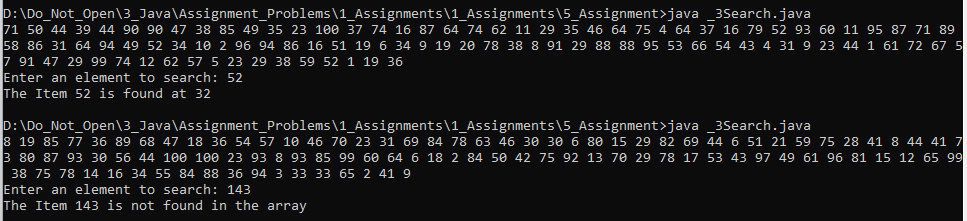
\includegraphics[width=0.8\textwidth]{3.png}
\end{center}

% 4

\section{}
\textbf{Task:} Create a procedure to insert a new employee (IN parameters).

\subsection{}
\begin{lstlisting}
delimiter //
create procedure add_emp(in emp_name varchar(50), in emp_sal decimal(10,2), in emp_dept varchar(30))
begin
    insert into employees (name, salary, department)
    values (emp_name, emp_sal, emp_dept);
end //
delimiter ;

call add_emp('sony', 43000, 'IT');

select * from employees;
\end{lstlisting}

\subsubsection{}
\begin{center}
    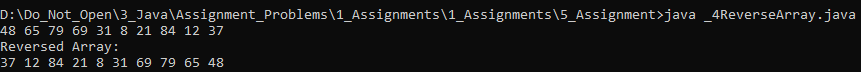
\includegraphics[width=0.8\textwidth]{4.png}
\end{center}

% 5

\section{}
\textbf{Task:} Create a procedure to insert a new department (IN parameters).

\subsection{}
\begin{lstlisting}
delimiter //
create procedure addDept(
    in d_name varchar(30),
    in loc varchar(30))
begin
    insert into departments(dept_name, location)
    values (d_name, loc);
end //
delimiter ;

call addDept('Physics', 'Hyderabad');

select * from departments;
\end{lstlisting}

\subsubsection{}
\begin{center}
    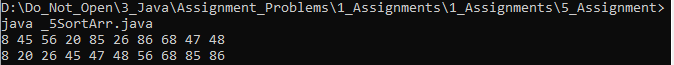
\includegraphics[width=0.8\textwidth]{5.png}
\end{center}

% 6

\section{}
\textbf{Task:} Create a procedure to delete an employee by name (IN parameter).

\subsection{}
\begin{lstlisting}
delimiter //
create procedure del_emp_name(in n varchar(50))
begin
    delete from employees
    where name = n;
end //
delimiter ;

call del_emp_name('vinod');

select * from employees;
\end{lstlisting}

\subsubsection{}
\begin{center}
    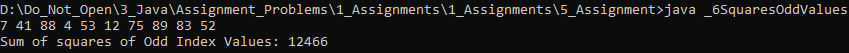
\includegraphics[width=0.8\textwidth]{6.png}
\end{center}

% 7

\section{}
\textbf{Task:} Create a procedure to change an employee’s department (IN parameters).

\subsection{}
\begin{lstlisting}
delimiter //
create procedure empDeptChange(
	in e_id int,
    in dept varchar(30))
begin
	update employees
    set department = dept
    where emp_id = e_id;
end //
delimiter ;

call empDeptChange(3, 'CSE');

select * from employees;
\end{lstlisting}

\subsubsection{}
\begin{center}
    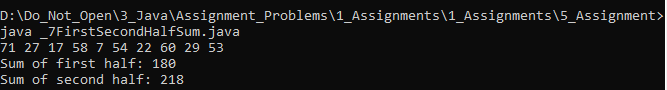
\includegraphics[width=0.8\textwidth]{7.png}
\end{center}

% 8

\section{}
\textbf{Task:} Create a procedure to get the highest salary (OUT parameter).

\subsection{}
\begin{lstlisting}
delimiter //
create procedure empHighestSalary(out h_sal decimal(10, 2))
begin
	select max(salary) into h_sal from employees;
end //
delimiter ;

call empHighestSalary(@highestSal);

select @highestSal as HighestSalary;
\end{lstlisting}

\subsubsection{}
\begin{center}
    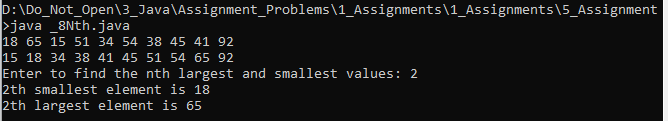
\includegraphics[width=0.8\textwidth]{8.png}
\end{center}

% 9

\section{}
\textbf{Task:} Create a procedure to get average salary (OUT parameter).

\subsection{}
\begin{lstlisting}
delimiter //
create procedure empAvgSal(out avgSal decimal(10, 2))
begin
	select avg(salary) into avgSal from employees;
end //
delimiter ;

call empAvgSal(@AvgSal);

select @AvgSal as EmployeesAverageSalary;
\end{lstlisting}

\subsubsection{}
\begin{center}
    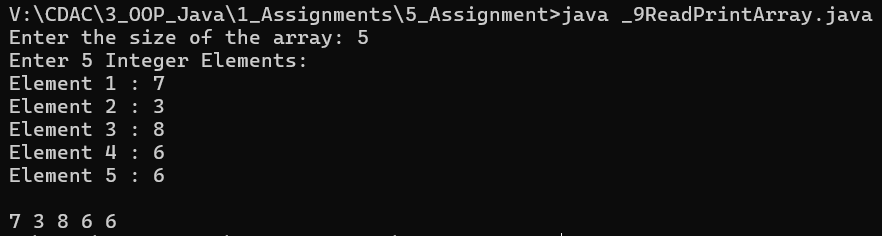
\includegraphics[width=0.8\textwidth]{9.png}
\end{center}

% 10

\section{}
\textbf{Task:} Create a procedure to get department count (OUT parameter).

\subsection{}
\begin{lstlisting}
 delimiter //
 create procedure deptCount(out d_count int)
 begin
	select count(*) into d_count from departments;
 end //
 delimiter ;
 
 call deptCount(@dept_count);
 
 select @dept_count as DepartmentCount;
 
 select * from  departments;
\end{lstlisting}

\subsubsection{}
\begin{center}
    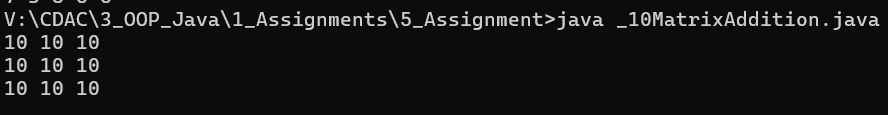
\includegraphics[width=0.8\textwidth]{10.png}
\end{center}

% 11

\section{}
\textbf{Task:} Create a procedure to get an employee’s name by ID (IN and OUT parameter).

\subsection{}
\begin{lstlisting}
delimiter //
create procedure getEmpName(in e_id int, out e_name varchar(50))
begin
	select name into e_name from employees where emp_id = e_id;
end //
delimiter ;

call getEmpName(5, @emp_name);

select @emp_name as EmployeeName;
\end{lstlisting}

\subsubsection{}
\begin{center}
    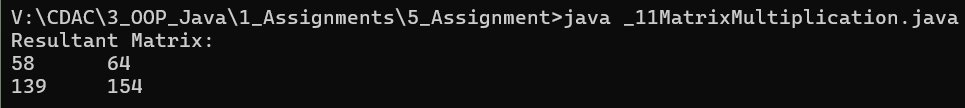
\includegraphics[width=0.8\textwidth]{11.png}
\end{center}

% 12

\section{}
\textbf{Task:} Create a procedure to increase salary of an employee by a given percentage (IN
parameters).

\subsection{}
\begin{lstlisting}
delimiter //
create procedure incEmpSal(in e_id int, in increase int)
begin
	update employees
    set salary = salary + (salary * (increase/100)) where emp_id = e_id;
end //
delimiter ;

call incEmpSal(5, 10);

select * from employees;
\end{lstlisting}

\subsubsection{}
\begin{center}
    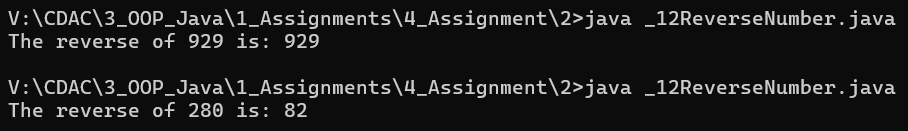
\includegraphics[width=0.8\textwidth]{12.png}
\end{center}

% 13

\section{}
\textbf{Task:} Create a procedure to add a bonus to an employee and return updated salary (INOUT parameter).

\subsection{}
\begin{lstlisting}
delimiter //
create procedure addBonusToEmployee(in e_id int, inout emp_sal decimal(10, 2), in bonus decimal(10, 2))
begin
	-- step 1: fetch current salary
	select salary into emp_sal 
    from employees where emp_id = e_id;
    
    -- step 2: add bonus
    
    set emp_sal = emp_sal + bonus;
    
    -- step 3: update employee salary
    update employees
    set salary = emp_sal
    where emp_id = e_id;
end //
delimiter ;

set @salary = 0;

call addBonusToEmployee(5, @salary, 25000);

select @salary as "Updated Salary";
\end{lstlisting}

\subsubsection{}
\begin{center}
    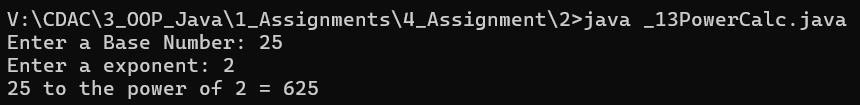
\includegraphics[width=0.8\textwidth]{13.png}
\end{center}

% 14

\section{}
\textbf{Task:} Create a procedure to move an employee to another department and return new
department name (INOUT parameter).

\subsection{}
\begin{lstlisting}
delimiter //
create procedure MoveEmployeeToDept(in e_id int, inout new_dept varchar(30))
begin
	update employees
    set department = new_dept
    where emp_id = e_id;
end //
delimiter ;

set @dept = 'dac';
call MoveEmployeeToDept(6, @dept);

select * from employees;
\end{lstlisting}

\subsubsection{}
\begin{center}
    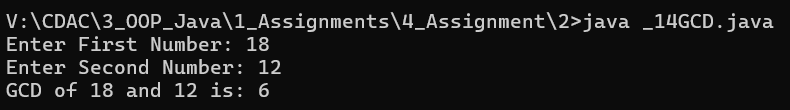
\includegraphics[width=0.8\textwidth]{14.png}
\end{center}

% 15

\section{}
\textbf{Task:} Create a procedure to change department location and return updated location (INOUT parameter).

\subsection{}
\begin{lstlisting}
delimiter //
create procedure changeDeptLoc(in d_id int, inout d_loc varchar(30))
begin
	update departments
    set location = d_loc
    where dept_id = d_id;
end //
delimiter ;

set @loc = 'Pune';
call changeDeptLoc(4, @loc);

select @loc as updated_location;

select * from departments;
\end{lstlisting}

\subsubsection{}
\begin{center}
    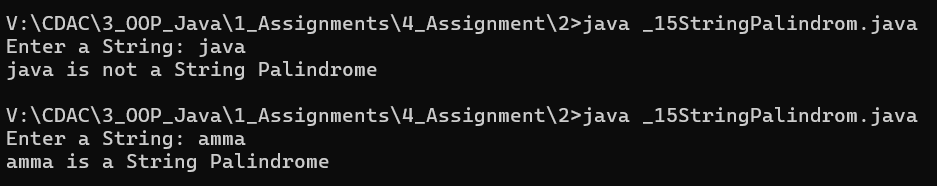
\includegraphics[width=0.8\textwidth]{15.png}
\end{center}

% 16

\section{}
\textbf{Task:} Create a procedure to show employees earning above a given salary (IN parameter).

\subsection{}
\begin{lstlisting}
delimiter //
create procedure empAboveSal(in sal decimal(10, 2))
begin
	select * from employees where salary > sal;
end //
delimiter ;

call empAboveSal(55000);
\end{lstlisting}

\subsubsection{}
\begin{center}
    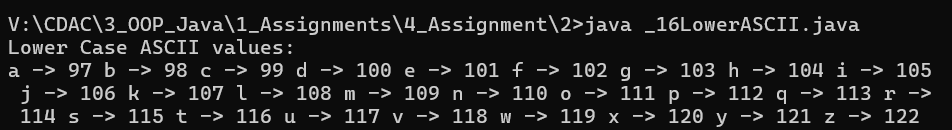
\includegraphics[width=0.8\textwidth]{16.png}
\end{center}

% 17

\section{}
\textbf{Task:} Create a procedure to show all departments in a specific location (IN parameter).

\subsection{}
\begin{lstlisting}
delimiter //
create procedure showDeptInLoc(in loc varchar(30))
begin
	select * from departments where location = loc;
end //
delimiter ;

call showDeptInLoc('Pune');
\end{lstlisting}

\subsubsection{}
\begin{center}
    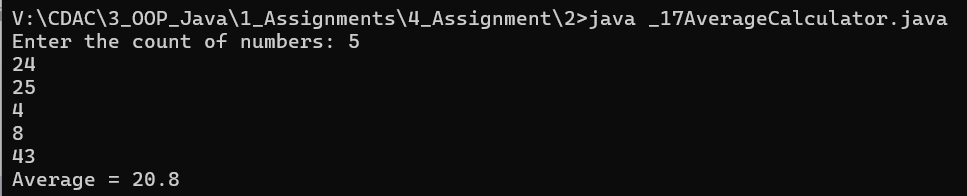
\includegraphics[width=0.8\textwidth]{17.png}
\end{center}

% 18

\section{}
\textbf{Task:} Create a procedure to delete a department by name (IN parameter).

\subsection{}
\begin{lstlisting}
delimiter //
create procedure delDeptByName(in d_name varchar(30))
begin
	delete from departments where dept_name = d_name;
end //
delimiter ;

call delDeptByName('Physics');

select * from departments;
\end{lstlisting}

\subsubsection{}
\begin{center}
    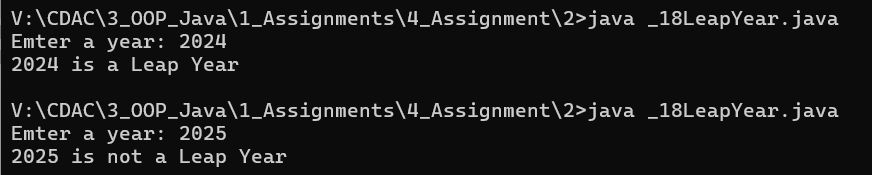
\includegraphics[width=0.8\textwidth]{18.png}
\end{center}

% 19

\section{}
\textbf{Task:} Create a procedure to find the total salary paid in a department (IN and OUT
parameter).

\subsection{}
\begin{lstlisting}
delimiter //
create procedure totalSalDeptWise(in d_name varchar(30), out t_sal decimal(10, 2))
begin
	select sum(salary) into t_sal from employees where department = d_name;
end //
delimiter ;

call totalSalDeptWise('IT', @totalSal);

select @totalSal as TotalSalary;

select * from employees;
\end{lstlisting}

\subsubsection{}
\begin{center}
    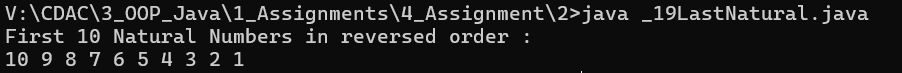
\includegraphics[width=0.8\textwidth]{19.png}
\end{center}

% 20

\section{}
\textbf{Task:} Create a procedure to find the minimum salary and return it (OUT parameter).

\subsection{}
\begin{lstlisting}
delimiter //
create procedure MinSal(out sal decimal(10, 2))
begin
	select min(salary) into sal
    from employees;
end //
delimiter ;

call MinSal(@minSalary);

select @minSalary as MinimumSalary;

select * from employees;
\end{lstlisting}

\subsubsection{}
\begin{center}
    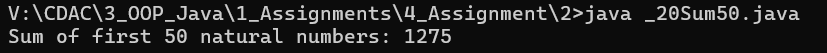
\includegraphics[width=0.8\textwidth]{20.png}
\end{center}


\end{document}
